\chapter{Présentation de l'entreprise}

\section{VideoStitch}
\subsection{Présentation générale}
\begin{wrapfigure}[6]{r}{7cm}
  \centering
  
\includegraphics[width=6cm]{images/videostitch-logo.jpg}
  \caption{Logo de VideoStitch}
\end{wrapfigure}
VideoStitch est une entreprise française d'édition de logiciels, qui conçoit et 
vend des logiciels de capture, de montage, de montage, de diffusion et de lecture 
de vidéos panoramiques à 360\degree. Elle s'intéresse par extension au marché de 
la réalité virtuelle.
Son site internet est à l'adresse suivante : \url{http://www.video-stitch.com/}.\\
C'est une Société à Actions Simplifiées (SAS) basée sur Paris, qui emploie moins
d'une dizaine de personnes actuellement. La plupart ayant été embauchés il y a 
quelques mois, c'est une société en forte croissance. 
Nicolas Burtey en est le président.

\subsection{L'équipe}
L'équipe est actuellement composée de 8 personnes et d'un nombre variable de 2 à 5 stagiaires.\\
Nicolas Burtey et Aksel Piran sont en charge de
la partie commerciale et marketing de l'entreprise. Ils consacrent également
du temps dans la recherche d'investisseurs et la présentation de l'entreprise dans
des salons ou des conférences. En outre, M. Burtey suit l'avancement des produits
en passant un jour ou deux dans la semaine avec l'équipe des développeurs.\\
Nicolas Lopez, Wieland Morgenstern et Henri Rebecq travaillent sur le c\oe ur du
projet, \cf{videostitch-sdk-section}, mettant au point algorithmes et nouvelles fonctionnalités.\\
Andrés Peralta, Julien Fond et Raphaël Lemoine travaillent quand à eux à la conception 
des trois autres produits de VideoStitch basés sur \nameref{videostitch-sdk-section}~: 
\cf{videostitch-studio-section}, \cf{vahana-vr-section}, \cf{videostitch-player-section}.\\
Liesbeth De Mey, stagiaire, est en charge de réaliser des \textit{screencast} et 
des tutoriels vidéos des produits de l'entreprise. Enfin, Jean Duthon et Marie
Chatelin, stagiaire UTCéens en TN09 également, sont en charge, respectivement,
de la \textit{QA}\footnote{\textit{Quality Assurance}} et de l'intégration continue
des quatre produits pour Jean, et d'assister l'équipe au développement des logiciels
pour Marie. Leurs rapports contiennent de plus amples détails sur le déroulé de 
leurs stages.

\subsection{Historique}
VideoStitch a été fondée par ce même Nicolas Burtey en janvier 2012.\\
Photographe diplômé de l'Ecole Lumière, s'étant fait connaître par la photo panoramique 
et la photo fish-eye, M. Burtey évolue par la suite dans le domaine de la vidéo panoramique.\\
\begin{wrapfigure}[6]{l}{6cm}
  \centering
  
\includegraphics[width=5cm]{images/loopin-logo.png}
  \caption{Logo de Loop'In}
\end{wrapfigure}
Il crée sa société de production vidéo, Loop'In, avec laquelle il réalise une 
certain nombre de vidéos panoramiques à 360\degree pour des boites de production (publicité essentiellement). 
Des exemples de ces vidéos sont disponibles à cette adresse : \url{http://www.loop-in.com/galerie/}.
La vidéo panoramique, étant alors un procédé très jeune encore inconnu du grand public, est 
lente et difficile à réaliser: beaucoup de tâches doivent être faites de manière 
manuelle et répétitive, avec des outils inadaptés car non prévus à cette utilisation.
Si la création de photos panoramiques et à 360\degree est aisée, il manque toutefois 
un logiciel complet et mature qui permetrait l'édition et le montage de vidéos paramiques.\\
\newline
M. Burtey décide alors de créer VideoStitch pour concevoir cet outil, un logiciel 
d'édition et de montage de vidéos panoramiques : VideoStitch Studio.
Quand ce logiciel atteint une version stable, en 2014, VideoStitch oriente alors 
ses efforts vers un nouveau logiciel, Vahana VR, permettant cette fois-ci une réalisation 
et une diffusion en direct de vidéos panoramiques à 360\degree.\\
Le but de la société est de permettre une réalisation aisée et de qualité de vidéos 
panoramiques à 360\degree, de la capture des images à la diffusion de la vidéo finale, 
en passant par sa réalisation complète.


\section{La vidéo 360}
\subsection{Du panorama à la vidéo 360}
Une image panoramique, ou panorama, est une superposition d'images qui sont assemblées
pour composer une vue bien plus large que ne le permet une image seule. La figure~ 
\ref{rochester-ny} présente un exemple d'assemblage d'un panorama.\\
Concrètement, avec un appareil photograhique, cela consiste à prendre plusieurs vues
successives en tournant l'appareil autour d'un axe entre deux clichés. 
Les photos obtenues forment ainsi une série d'un même sujet et doivent pouvoir 
se recouvrir en partie pour être ensuite assemblées en une seule image panoramique. 
Cet assemblage peut être réalisé avec directement par l'appareil, comme c'est le cas des 
téléphones portables, ou par un logiciel spécialisé, comme Photoshop\cite{photomerge} 
ou PTgui\cite{PTgui}.
\begin{figure}
  \centering
  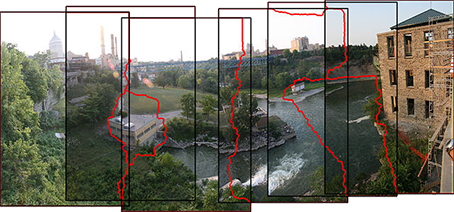
\includegraphics[width=11cm]{images/rochester-ny.png}
  \caption{Exemple d'assemblage de panorama avec détection des zones de recouvrement\cite{RochesterNY}}
  \label{rochester-ny}
\end{figure}
\newline
La vidéo panoramique consiste à filmer avec plusieurs caméras en même temps, chacune
capturant une partie du panorama, pour assembler les images capturées en une seule
vidéo par le même princique que la photo panoramique.\\
Avec suffisament de caméras, il est possible de couvrir un angle de prise de vue 
de 360\degree à l'horizontale et de 180\degree à la verticale. Le panorama créé
forme alors une sphère virtuelle, comme le montre la figure~\ref{camera-projection}. 
C'est ce qu'on appelle la vidéo 360.
\begin{figure}
  \centering
  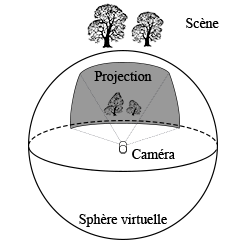
\includegraphics[width=6.5cm]{images/camera-projection.png}
  \caption{Exemple d'une scène filmée avec une caméra}
  \label{camera-projection}
\end{figure}
\newline
Cependant, comme le montre la figure~\ref{rochester-ny}, un panorama reste une image
$-$ ou une vidéo $-$, c'est-à-dire une matrice plane consistuée de pixels\footnote{Pour
 \enquote{picture element}}. Or une vidéo 360 représentant une sphère virtuelle, ou
plutôt sa surface, elle sera nécessairement une \emph{projection} de cette sphère, 
c'est-à-dire une correspondance mathématique entre cette surface en 3 dimensions 
et cette vidéo plane\cite{projection-cartographique}.\\
Dans la vidéo 360, la projection la plus utilisée est la projection équirectangulaire\cite{what-is-equirectangular}.
Un exemple en est le planisphère terrestre, où après une projection cylindrique équirectangulaire
sur la figure~\ref{projection-cylindrique} le plan est déroulé pour obtenir le 
planisphère de la figure~\ref{planisphère}.
\begin{figure}
  \centering
  \begin{minipage}[t]{0.35\textwidth}
    \centering
    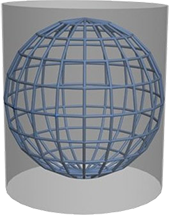
\includegraphics[width=3.4cm]{images/projection-cylindrique.png}
    \captionof{figure}{Schéma d'une projection équirectangulaire\cite{projection-cylindrique}}
    \label{projection-cylindrique}
  \end{minipage}%
  \hspace{0.04\textwidth}
  \begin{minipage}[t]{0.6\textwidth}
    \centering
    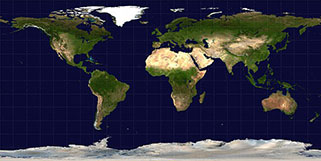
\includegraphics[width=8.5cm]{images/equirectangular-projection.jpg}
    \captionof{figure}{Projection équirectangulaire de la Terre\cite{planisphere}}
    \label{planisphère}
  \end{minipage}
\end{figure}
\newline
Un lecteur vidéo 360 est alors nécessaire pour lire correctement la vidéo~: 
il va reconstruire la sphère, pour y projetter le panorama et y placer le
spectateur au centre de cette sphère. Dès lors, le spectateur peut déplacer le 
regard tout autour de lui pour embrasser le panorama : on entre dans le champs de 
la réalité virtuelle\footnote{La réalité virtuelle est ici comprise dans son sens
  de \enquote{Simulation sensorielle immersive de la réalité}\cite{definition-rv}}.

\subsection{Le marché de la vidéo 360}
Si les années 2000 ont vu la démocratisation des appareils photographiques numériques,
les années 2010 voient l'émergence des caméras numériques Haute 
Définition\footnote{Définition d'image de 1920x1080 pixels} bon marché, comme les GoPro,
et des écrans 4K\footnote{Définition d'image de 4096x2160 pixels}. De plus les capacités
informatiques grand public permettent désormais de stocker et traiter plusieurs 
vidéos HD en même temps.\\
Dès lors la vidéo 360 peut se développer, son coût technique
étant accessible, et le marché, bien qu'encore restreint et méconnu du public,
est un plein développement et présente déjà de très nombreux concurrents. Jaunt,
entreprise américaine créée en mai 2013 a, par exemple, déjà levé 35 millions
de dollars de fonds d'investissement\cite{jaunt-fundings}.\\
Les grandes entreprises comme Facebook\cite{facebook-vr}, Samsung\cite{samsung-vr}, 
Microsoft\cite{microsoft-vr} ou Google\cite{google-vr} suivent de
très près ce marché, notamment pour concevoir des produits de réalité virtuelle 
ou de réalité augmentée, qui progressivement vont s'installer dans les usages
du public, tout comme l'ont fait auparavant les ordinateurs portables, les téléphones mobiles
et les tablettes numériques.\\

\section{Produits et stratégies de l'entreprise}
Par rapport à ce marché, VideoStitch se positionne aujourd'hui comme un challenger
et propose actuellement quatre produits\cite{videostitch-products}.
\subsection{VideoStitch Studio}
\label{videostitch-studio-section}
\label{videostitch-studio}
%\begin{wrapfigure}[5]{r}{5cm}
%  \centering
%  
\includegraphics[width=4cm]{images/studio.png}
%  \caption{Logo de VideoStitch Studio}
%\end{wrapfigure}
Premier logiciel de l'entreprise, sortis en version stable en 2013 pour Windows, Mac OS X et Linux,
il permet une utilisation post-production de captures vidéos 360, c'est-à-dire 
la conception de vidéos 360. Le \textit{workflow} de travail avec le logiciel est le suivant : 
\subsubsection{Importation des vidéos}
\label{importation-videos}
Le cas le plus commun est de capturer la vidéo 360 à l'aide de 6 caméras GoPro 
installées sur une monture spécialisée\footnote{Aussi appellée \textit{rig}} comme sur la figure~\ref{rig}. 
Les caméras sont configurées pour filmer en HD, et, munies de leurs optiques 
d'origine, six sont nécessaires pour filmer toute la sphère du panorama.
\begin{figure}
  \centering
  \begin{minipage}[b]{0.3\textwidth}
    \centering
    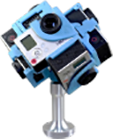
\includegraphics[width=3cm]{images/rig.png}
    \caption{Une monture 360}
    \label{rig}
  \end{minipage}%
  \hspace{0.04\textwidth}
  \begin{minipage}[b]{0.65\textwidth}
    \centering
    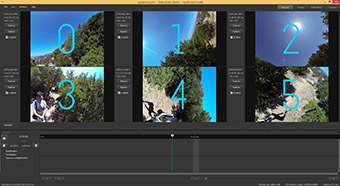
\includegraphics[width=9cm]{images/studio-sources-numeros.jpg}
    \caption{Les 6 fichiers vidéos source numérotés importés dans Studio}
    \label{importation}
  \end{minipage}
\end{figure}

\subsubsection{Synchronisation des vidéos}
Lors de la capture, les caméras sont bien souvent démarées en décalées. Il s'agit
donc de resynchroniser les vidéos enregistrées.\\
Pour cela, la méthode la plus pratique est le \textit{motion},
où le logiciel analyse les mouvements de chaque vidéo : en effet les caméras étant fixées
sur la même monture, elles ont donc décris les mêmes mouvements dans l'espace, mais 
en décalé sur les vidéos.

\subsubsection{Calibration}
A cette étape est reconstituée la sphère; ce qui consiste à retrouver la 
position relative de chaque caméra par rapport à la monture.\\
A un même instant des vidéos, choisis par l'utilisateur, le logiciel trouve des
points de contrôle entre les images des différentes caméras, c'est-à-dire des
points identiques de la scène présents sur au moins deux images. C'est ici que les 
zones de recouvrements entre les images trouvent leur importance.\\
Une fois les points trouvés, les vidéos peuvent être superposées et être assemblées
\footnote{C'est ce qu'on appelle le \textit{stitch}}.
\begin{figure}
  \centering
  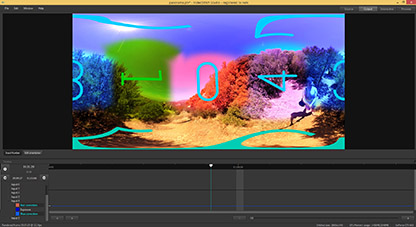
\includegraphics[width=11cm]{images/studio-output-angles-numeros.jpg}
  \caption{Équirectangulaire avec angle de capture colorisés et numéros des 6 sources} 
\end{figure}

\subsubsection{Correction d'exposition}
Chaque caméra ayant filmé dans une direction, les différentes vidéos auronts chacune 
des expositions différentes. De même, les balances des blancs peuvent différer
entre les vidéos. Le logiciel corrige localement ces deux paramètres pour homogéiniser
le panorama final.

\subsubsection{Stabilisation}
La stabilisation consiste à  lisser les micro-mouvements des vidéos, qui ont 
pu se produire lors de la capture, par exemple si la monture s'est déplacée dans l'espace lors
de l'enregistrement. Cette étape est nécessaire : regarder dans un casque de réalité
virtuelle une vidéo non stabilisée est très désagréable.

\subsubsection{Correction de l'orientation}
Il s'agit simplement ici de redonner sens aux notions de haut et de bas dans la 
vidéo 360. En effet, si la calibration a permis de retrouver les positions des 
caméras par rapport à la monture, le logiciel n'a aucune information sur la position
de la monture par rapport à la scène. Comme le montre la figure~\ref{orientation},
la correction s'effectue par un clic de souris enfoncé
et glissé jusqu'à déplacer l'équirectangulaire dans la position voulue. Un bon résultat
est obtenu quand l'horizon est redressé.
\begin{figure}
  \centering
  \begin{minipage}{0.45\textwidth}
    \centering
    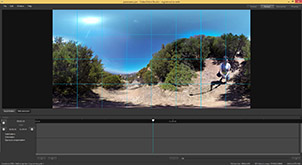
\includegraphics[width=8.0cm]{images/studio-output-exposure-grid.jpg}
  \end{minipage}%
  \hspace{0.08\textwidth}
  \begin{minipage}{0.45\textwidth}
    \centering
    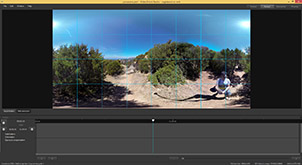
\includegraphics[width=8.0cm]{images/studio-output-exposure-grid-oriented.jpg}
  \end{minipage}
  \caption{Correction de l'orientation : l'horizon est redressé}
  \label{orientation}
\end{figure}

\subsubsection{Exportation}
\label{exportation}
Enfin, la vidéo 360 peut être exportée sous la forme d'un équirectangulaire, avec
possibilité d'intégrer le son d'unes des caméras.

\begin{figure}
  \centering
  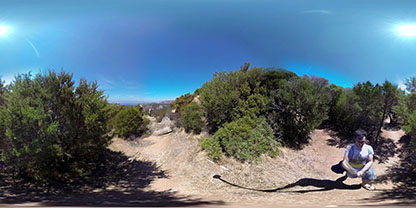
\includegraphics[width=11cm]{images/studio-equirectangular.jpg}
  \caption{Équirectangulaire final} 
\end{figure}

\subsection{Vahana VR}
\label{vahana-vr-section}
%\begin{wrapfigure}[7]{r}{4cm}
%  \centering
%  
\includegraphics[width=3cm]{images/vahanavr.png}
%  \caption{Logo de Vahana VR}
%\end{wrapfigure}
Ce nouveau logiciel, dont la sortie stable devrait s'effectuer en février 2015 uniquement sous Windows,
permet de réaliser le travail de Studio en temps réel, ainsi qu'une diffusion
de l'export en \textit{streaming live}. Les vidéos sont ici directement capturées des
caméras via des cartes d'acquisitions, et après une étape de calibration, sont
assemblées automatiquement. Le logiciel assure lui-même la bonne synchronisation
des vidéos.\\
Le panorama peut être alors exporté sur différents flux en même temps : 
streaming RTMP, via une carte d'acquisition pour une sortie HDMI ou SDI, sur le
disque dur. Ce logiciel ouvre la possibilité du \textit{streaming} 360 à des événéments 
\textit{live}, comme les concerts, le sport, les défilés ou encore les conférences.
\begin{figure}
  \centering
  \begin{minipage}{0.45\textwidth}
    \centering
    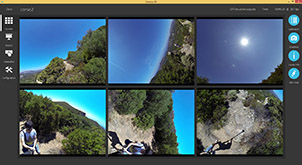
\includegraphics[width=8.0cm]{images/vahana-vr-sources.jpg}
    \caption{6 entrées vidéos sur Vahana VR}
  \end{minipage}%
  \hspace{0.08\textwidth}
  \begin{minipage}{0.45\textwidth}
    \centering
    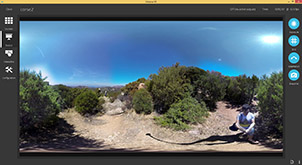
\includegraphics[width=8.0cm]{images/vahana-vr-output.jpg}
    \caption{Équirectangulaire assemblé après calibration des vidéos}
  \end{minipage}
\end{figure}

\subsection{VideoStitch Player}
\label{videostitch-player-section}
%\begin{wrapfigure}[7]{r}{4cm}
%  \centering
%  
\includegraphics[width=3cm]{images/player.png}
%  \caption{Logo de VideoStitch Player}
%\end{wrapfigure}
C'est un lecteur de vidéo 360, développé par Alexis Pontin lors de son TN10 au précédent
semestre de Printemps 2014, sous Windows, Mac OS X et Linux. Le logiciel permet de lire des vidéos 360 depuis un 
fichier vidéo équirectangulaire ou depuis un flux RTMP de Vahana VR. La vidéo peut-être
lue dans un mode interactif avec utilisation de la souris pour déplacer le regard,
ou en mode Oculus Rift, où la vidéo est projetée dans le casque de réalité virtuelle.
L'utilisation du casque est tout à fait naturelle : le casque disposant d'un gyroscope
et d'un accéléromètre, il renvoie au lecteur la position de la tête de l'utilisateur.\\
Regarder une vidéo avec l'Oculus Rift depuis un flux RTMP de Vahana VR est une 
expérience toute à fait singulière : le regard est téléporté à la place de la caméra.
Il est possible de se voir soi-même en direct, créant un dédoublement du corps et du regard
\footnote{Une démonstration est disponible en ligne : \url{https://www.youtube.com/watch?v=fQGLqAg0eRU}}.
\begin{figure}
  \centering
  \begin{minipage}{0.45\textwidth}
     \centering
     \caption{Vue interactive dans le Player de l'équirectangulaire exporté}
  \end{minipage}%
  \hspace{0.08\textwidth}
  \begin{minipage}{0.45\textwidth}
    \centering
    \caption{Illustration d'un visionnage d'une vidéo 360 dans un Oculus Rift}
  \end{minipage}
\end{figure}

\subsection{VideoStitch SDK}
\label{videostitch-sdk-section}
\begin{wrapfigure}[7]{r}{6cm}
  \centering
  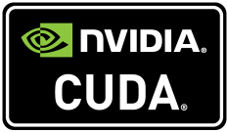
\includegraphics[width=6cm]{images/cuda-logo.jpg}
  \caption{CUDA}
\end{wrapfigure}
Ces applications s'appuient toute trois sur une librairie développée séparément,
en C++/CUDA. C'est cette librairie qui implémente et éxecute tous les algorithmes
de synchronisation, calibration, gestions des flux vidéos et audio et corrections
vidéos.
Toutes ces opérations sont très coûteuses en temps de calcul. C'est pourquoi
la techologie CUDA de nVidia est utilisée pour exploiter le potentiel de la carte
graphique\footnote{Ou \textit{GPU} pour \textit{Graphics Processing Unit}}. 
En effet un \textit{GPU} est composé de milliers de c\oe urs fonctionnant en parallèles.
Or la librairie travaille sur des images vidéos, c'est-à-dire des matrices de pixels,
avec des calculs massivement parallélisable\cite{videostitch-cuda}.\\
\newline
Cette librairie est distribuée sous forme de \textit{SDK}\footnote{\textit{Software Development Kit}}, sous Windows, Mac OS X et Linux, 
pour des clients souhaitant concevoir leur propre caméra ou un logiciel exploitant
les opérations \textit{stitch}.

\subsection{Stratégies}
Si VideoStitch est pendant un certain temps restée une petite start-up développant
un outil de post-production pour vidéos 360 
\footnote{VideoStitch Studio, section \ref{videostitch-studio}}, 
l'entreprise ambitionne désormais d'être le leader du marché.\\
Le marché est encore jeune, mais se décidera certainement en 2015 et s'alignera
probablement sur un leader. La technologie sera suffisament mature, et des rachats
par de grands groupe sont probable, comme cela s'est produit dans le marché de la
réalité virtuelle en 2014, avec le rachat de l'Oculus Rift par Facebook 
\cite{facebook-vr} par exemple.\\
Ce marché permettra également l'émergence de nouveaux contenus 360 pour les appareils
de réalité virtuelle, comme par exemple du cinéma ou de la télévision 360.
VideoStitch Studio et Vahana VR sont déjà des outils pertinents pour créer ces 
nouveaux types de contenus, en particulier Vahana VR pour le streaming 360 en direct.
Pour cela il est important que Vahana VR soit le premier produit sur le marché
de la 360 \textit{live} et qu'il en prenne la tête~: c'est l'opportunité pour VideoStitch
de \enquote{décoller}.\\
\newline
Cependant d'autres pistes seront ensuite à développer. En effet, avec ces quatre produits
l'entreprise se destinerait actuellement à une position de service pour des entreprises de production
de vidéo 360 d'une part et à des entreprises développant des services 360 pour le
public d'une autre part. Le développement d'une solution complète incluant une 
caméra permettrait de dépasser cette position et atteindre le segment du grand public, incluant
les entreprises non spécialisées dans la production vidéo.
De plus, cela assurerait de grandes rentrées d'argent et donnerait à l'entreprise des
moyens à ses ambitions.
